% Fig. 7 - MSG3 Resolution Procedure (design-level decision tree)
% Design-level: decisions are conceptual questions, not code expressions
% Compile: pdflatex fig7_decision_tree.tex
\documentclass[border=8pt]{standalone}
\usepackage{amsmath}
\usepackage{tikz}
\usetikzlibrary{arrows.meta, positioning, shapes.geometric, calc}

\begin{document}
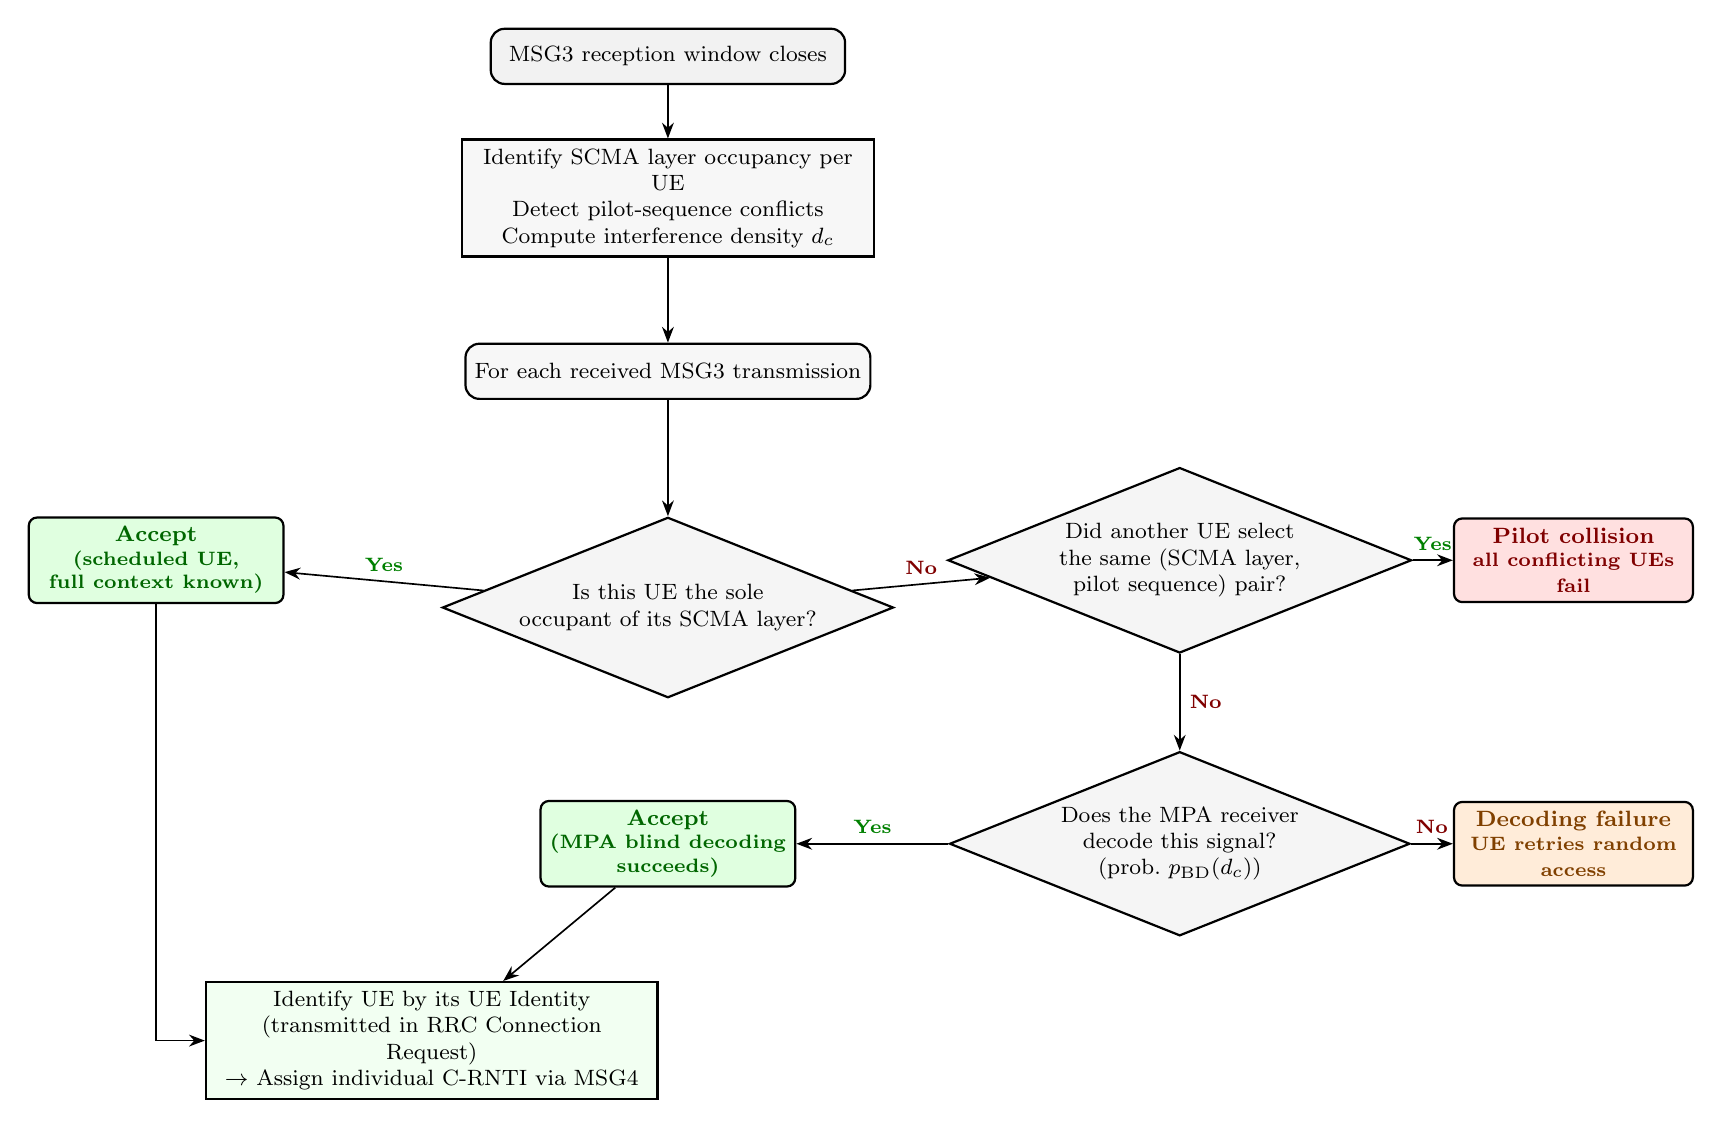
\begin{tikzpicture}[
    >=Stealth,
    font=\footnotesize,
    startstop/.style={draw, rectangle, rounded corners=5pt,
        minimum width=4.5cm, minimum height=0.7cm, fill=black!5, thick},
    process/.style={draw, rectangle, minimum width=4.5cm,
        minimum height=0.7cm, fill=black!3, thick=0.4pt},
    decision/.style={draw, diamond, aspect=2.5, inner sep=2pt,
        fill=black!4, align=center, thick=0.4pt},
    accept/.style={draw, rectangle, rounded corners=3pt,
        minimum width=2.8cm, minimum height=0.8cm,
        fill=green!12, text=green!40!black, font=\footnotesize\bfseries,
        align=center, thick=0.4pt},
    reject/.style={draw, rectangle, rounded corners=3pt,
        minimum width=2.8cm, minimum height=0.8cm,
        fill=red!12, text=red!50!black, font=\footnotesize\bfseries,
        align=center, thick=0.4pt},
    retry/.style={draw, rectangle, rounded corners=3pt,
        minimum width=2.8cm, minimum height=0.8cm,
        fill=orange!15, text=orange!50!black, font=\footnotesize\bfseries,
        align=center, thick=0.4pt},
    arrow/.style={->, semithick},
    yeslbl/.style={font=\scriptsize\bfseries, text=green!50!black},
    nolbl/.style={font=\scriptsize\bfseries, text=red!50!black},
]

% === Start ===
\node[startstop] (start) at (3, 0) {MSG3 reception window closes};

% === Preprocessing (design-level: verbs) ===
\node[process] (prep) at (3, -1.8) {\parbox{5cm}{\centering
    Identify SCMA layer occupancy per UE\\
    Detect pilot-sequence conflicts\\
    Compute interference density $d_c$
}};
\draw[arrow] (start) -- (prep);

% === For each entry ===
\node[startstop, fill=black!3] (foreach) at (3, -4.0)
    {For each received MSG3 transmission};
\draw[arrow] (prep) -- (foreach);

% === Decision 1: Sole occupant of SCMA layer? ===
\node[decision] (d1) at (3, -7.0)
    {\footnotesize Is this UE the sole\\occupant of its SCMA layer?};
\draw[arrow] (foreach) -- (d1);

% === YES: Scheduled (left) ===
\node[accept] (sched) at (-3.5, -6.4) {\parbox{3cm}{\centering
    Accept\\[-1pt]
    {\scriptsize (scheduled UE,}\\[-1pt]
    {\scriptsize full context known)}}};
\draw[arrow] (d1) -- node[yeslbl, above] {Yes} (sched);

% === NO: Decision 2 (right) ===
\node[decision] (d2) at (9.5, -6.4)
    {\footnotesize Did another UE select\\the same (SCMA layer,\\pilot sequence) pair?};
\draw[arrow] (d1) -- node[nolbl, above] {No} (d2);

% === YES: Pilot collision (far right) ===
\node[reject] (coll) at (14.5, -6.4) {\parbox{2.8cm}{\centering
    Pilot collision\\[-1pt]
    {\scriptsize all conflicting UEs fail}}};
\draw[arrow] (d2) -- node[yeslbl, above] {Yes} (coll);

% === NO: MPA decoding (below d2) ===
\node[decision] (d3) at (9.5, -10.0)
    {\footnotesize Does the MPA receiver\\decode this signal?\\(prob.\ $p_{\text{BD}}(d_c)$)};
\draw[arrow] (d2) -- node[nolbl, right] {No} (d3);

% === YES: MPA accept ===
\node[accept] (mpasuc) at (3, -10.0) {\parbox{3cm}{\centering
    Accept\\[-1pt]
    {\scriptsize (MPA blind decoding}\\[-1pt]
    {\scriptsize succeeds)}}};
\draw[arrow] (d3) -- node[yeslbl, above] {Yes} (mpasuc);

% === NO: Decoding failure ===
\node[retry] (mpaf) at (14.5, -10.0) {\parbox{2.8cm}{\centering
    Decoding failure\\[-1pt]
    {\scriptsize UE retries random access}}};
\draw[arrow] (d3) -- node[nolbl, above] {No} (mpaf);

% === Post-accept outcome ===
\node[process, fill=green!5] (grp) at (0, -12.5) {\parbox{5.5cm}{\centering
    Identify UE by its UE Identity\\
    (transmitted in RRC Connection Request)\\
    $\rightarrow$ Assign individual C-RNTI via MSG4
}};
\draw[arrow] (sched.south) |- (grp.west);
\draw[arrow] (mpasuc) -- (grp);

\end{tikzpicture}
\end{document}
